% Options for packages loaded elsewhere
\PassOptionsToPackage{unicode}{hyperref}
\PassOptionsToPackage{hyphens}{url}
\PassOptionsToPackage{dvipsnames,svgnames,x11names}{xcolor}
%
\documentclass[
  letterpaper,
  DIV=11,
  numbers=noendperiod]{scrartcl}

\usepackage{amsmath,amssymb}
\usepackage{lmodern}
\usepackage{iftex}
\ifPDFTeX
  \usepackage[T1]{fontenc}
  \usepackage[utf8]{inputenc}
  \usepackage{textcomp} % provide euro and other symbols
\else % if luatex or xetex
  \usepackage{unicode-math}
  \defaultfontfeatures{Scale=MatchLowercase}
  \defaultfontfeatures[\rmfamily]{Ligatures=TeX,Scale=1}
\fi
% Use upquote if available, for straight quotes in verbatim environments
\IfFileExists{upquote.sty}{\usepackage{upquote}}{}
\IfFileExists{microtype.sty}{% use microtype if available
  \usepackage[]{microtype}
  \UseMicrotypeSet[protrusion]{basicmath} % disable protrusion for tt fonts
}{}
\makeatletter
\@ifundefined{KOMAClassName}{% if non-KOMA class
  \IfFileExists{parskip.sty}{%
    \usepackage{parskip}
  }{% else
    \setlength{\parindent}{0pt}
    \setlength{\parskip}{6pt plus 2pt minus 1pt}}
}{% if KOMA class
  \KOMAoptions{parskip=half}}
\makeatother
\usepackage{xcolor}
\setlength{\emergencystretch}{3em} % prevent overfull lines
\setcounter{secnumdepth}{-\maxdimen} % remove section numbering
% Make \paragraph and \subparagraph free-standing
\ifx\paragraph\undefined\else
  \let\oldparagraph\paragraph
  \renewcommand{\paragraph}[1]{\oldparagraph{#1}\mbox{}}
\fi
\ifx\subparagraph\undefined\else
  \let\oldsubparagraph\subparagraph
  \renewcommand{\subparagraph}[1]{\oldsubparagraph{#1}\mbox{}}
\fi


\providecommand{\tightlist}{%
  \setlength{\itemsep}{0pt}\setlength{\parskip}{0pt}}\usepackage{longtable,booktabs,array}
\usepackage{calc} % for calculating minipage widths
% Correct order of tables after \paragraph or \subparagraph
\usepackage{etoolbox}
\makeatletter
\patchcmd\longtable{\par}{\if@noskipsec\mbox{}\fi\par}{}{}
\makeatother
% Allow footnotes in longtable head/foot
\IfFileExists{footnotehyper.sty}{\usepackage{footnotehyper}}{\usepackage{footnote}}
\makesavenoteenv{longtable}
\usepackage{graphicx}
\makeatletter
\def\maxwidth{\ifdim\Gin@nat@width>\linewidth\linewidth\else\Gin@nat@width\fi}
\def\maxheight{\ifdim\Gin@nat@height>\textheight\textheight\else\Gin@nat@height\fi}
\makeatother
% Scale images if necessary, so that they will not overflow the page
% margins by default, and it is still possible to overwrite the defaults
% using explicit options in \includegraphics[width, height, ...]{}
\setkeys{Gin}{width=\maxwidth,height=\maxheight,keepaspectratio}
% Set default figure placement to htbp
\makeatletter
\def\fps@figure{htbp}
\makeatother

\usepackage{booktabs}
\usepackage{longtable}
\usepackage{array}
\usepackage{multirow}
\usepackage{wrapfig}
\usepackage{float}
\usepackage{colortbl}
\usepackage{pdflscape}
\usepackage{tabu}
\usepackage{threeparttable}
\usepackage{threeparttablex}
\usepackage[normalem]{ulem}
\usepackage{makecell}
\usepackage{xcolor}
\usepackage{amsmath}
\usepackage{caption}
\KOMAoption{captions}{tableheading}
\makeatletter
\makeatother
\makeatletter
\makeatother
\makeatletter
\@ifpackageloaded{caption}{}{\usepackage{caption}}
\AtBeginDocument{%
\ifdefined\contentsname
  \renewcommand*\contentsname{Table of contents}
\else
  \newcommand\contentsname{Table of contents}
\fi
\ifdefined\listfigurename
  \renewcommand*\listfigurename{List of Figures}
\else
  \newcommand\listfigurename{List of Figures}
\fi
\ifdefined\listtablename
  \renewcommand*\listtablename{List of Tables}
\else
  \newcommand\listtablename{List of Tables}
\fi
\ifdefined\figurename
  \renewcommand*\figurename{Figure}
\else
  \newcommand\figurename{Figure}
\fi
\ifdefined\tablename
  \renewcommand*\tablename{Table}
\else
  \newcommand\tablename{Table}
\fi
}
\@ifpackageloaded{float}{}{\usepackage{float}}
\floatstyle{ruled}
\@ifundefined{c@chapter}{\newfloat{codelisting}{h}{lop}}{\newfloat{codelisting}{h}{lop}[chapter]}
\floatname{codelisting}{Listing}
\newcommand*\listoflistings{\listof{codelisting}{List of Listings}}
\makeatother
\makeatletter
\@ifpackageloaded{caption}{}{\usepackage{caption}}
\@ifpackageloaded{subcaption}{}{\usepackage{subcaption}}
\makeatother
\makeatletter
\@ifpackageloaded{tcolorbox}{}{\usepackage[many]{tcolorbox}}
\makeatother
\makeatletter
\@ifundefined{shadecolor}{\definecolor{shadecolor}{rgb}{.97, .97, .97}}
\makeatother
\makeatletter
\makeatother
\ifLuaTeX
  \usepackage{selnolig}  % disable illegal ligatures
\fi
\IfFileExists{bookmark.sty}{\usepackage{bookmark}}{\usepackage{hyperref}}
\IfFileExists{xurl.sty}{\usepackage{xurl}}{} % add URL line breaks if available
\urlstyle{same} % disable monospaced font for URLs
\hypersetup{
  pdftitle={American Samoa Model Checks},
  pdfauthor={Marc Nadon and Meg Oshima},
  colorlinks=true,
  linkcolor={blue},
  filecolor={Maroon},
  citecolor={Blue},
  urlcolor={Blue},
  pdfcreator={LaTeX via pandoc}}

\title{American Samoa Model Checks}
\author{Marc Nadon and Meg Oshima}
\date{2022-12-16}

\begin{document}
\maketitle
\ifdefined\Shaded\renewenvironment{Shaded}{\begin{tcolorbox}[enhanced, frame hidden, breakable, sharp corners, boxrule=0pt, interior hidden, borderline west={3pt}{0pt}{shadecolor}]}{\end{tcolorbox}}\fi

\textbf{This is a summary report for the LUKA base model run.}

\hypertarget{model-output}{%
\section{Model Output}\label{model-output}}

\hypertarget{input-data}{%
\paragraph{Input Data}\label{input-data}}

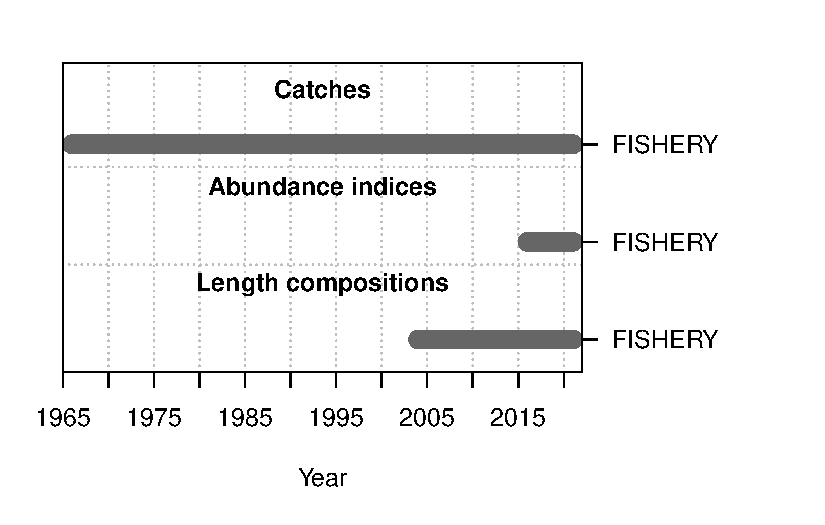
\includegraphics{LUKA_50_Base_model_diags_report_files/figure-pdf/dataplot-1.pdf}

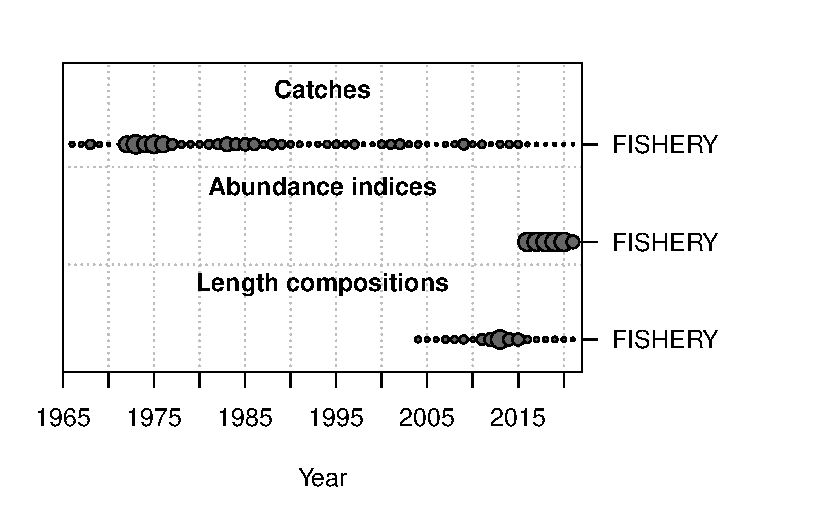
\includegraphics{LUKA_50_Base_model_diags_report_files/figure-pdf/dataplot-2.pdf}

\hypertarget{convergence-check}{%
\paragraph{Convergence Check}\label{convergence-check}}

\begin{verbatim}
  Converged     MaxGrad
1      TRUE 2.53274e-05
\end{verbatim}

\begin{verbatim}
[1] "1 NOTE:  Max data length bin: 28  < max pop len bins: 31; so will accumulate larger pop len bins"
[2] "2 Forecast F capped by max possible F from control file: 2.9"                                    
[3] "3 Forecast F capped by max possible F from control file: 2.9"                                    
[4] "N warnings: 3"                                                                                   
\end{verbatim}

\hypertarget{fit-to-model}{%
\paragraph{Fit to Model}\label{fit-to-model}}

\hypertarget{cpue}{%
\subsubsection{CPUE}\label{cpue}}

\begin{longtable}{lrr}
\toprule
Fleet & RMSE.perc & Nobs \\ 
\midrule
FISHERY & 21.9 & 6 \\ 
Combined & 21.9 & 6 \\ 
\bottomrule
\end{longtable}

\begin{figure}

{\centering 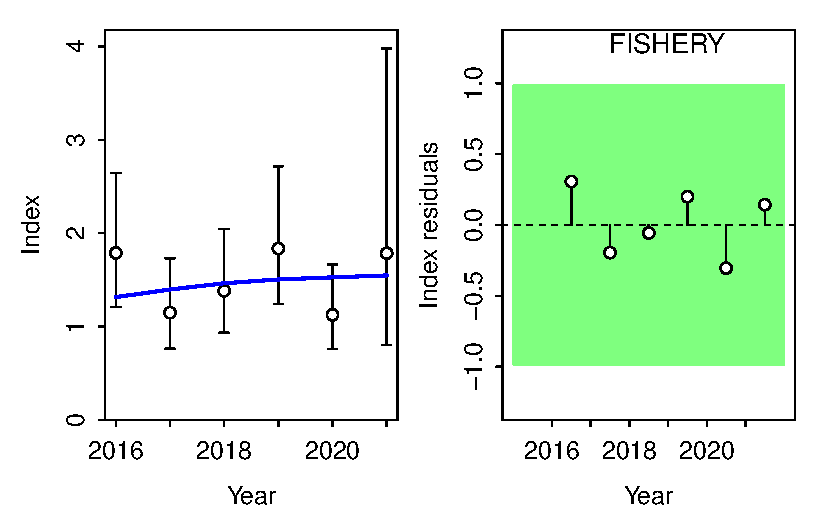
\includegraphics{LUKA_50_Base_model_diags_report_files/figure-pdf/indexfits-1.pdf}

}

\end{figure}

\hypertarget{length-comp}{%
\subsubsection{Length Comp}\label{length-comp}}

\begin{longtable}{lrr}
\toprule
Fleet & RMSE.perc & Nobs \\ 
\midrule
FISHERY & 1.3 & 18 \\ 
Combined & 1.3 & 18 \\ 
\bottomrule
\end{longtable}

\begin{figure}

\begin{minipage}[t]{0.50\linewidth}

{\centering 

\begin{verbatim}
         w         lo         hi 
0.14420929 0.07921066 0.55573995 
\end{verbatim}

}

\end{minipage}%
%
\begin{minipage}[t]{0.50\linewidth}

{\centering 

\begin{verbatim}
    Index runs.p   test   sigma3.lo  sigma3.hi type
1 FISHERY  0.135 Passed -0.02912284 0.02912284  len
\end{verbatim}

}

\end{minipage}%
\newline
\begin{minipage}[t]{0.50\linewidth}

{\centering 

\raisebox{-\height}{

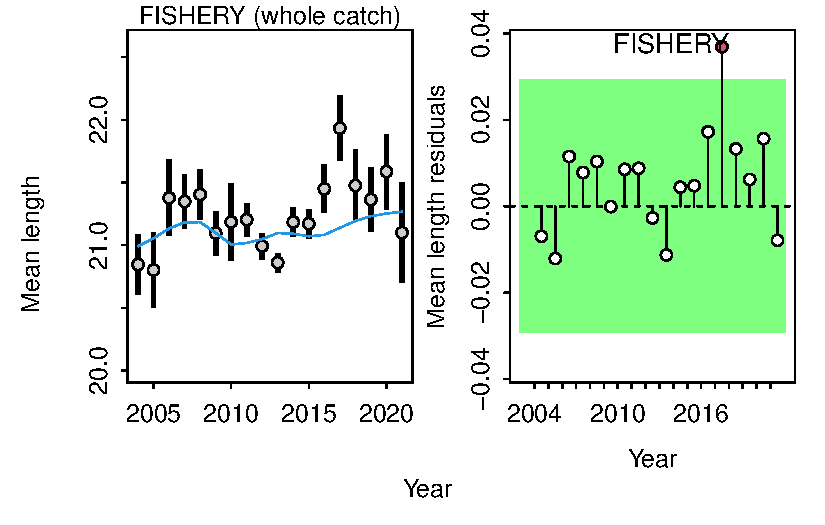
\includegraphics{LUKA_50_Base_model_diags_report_files/figure-pdf/lenfits-1.pdf}

}

}

\end{minipage}%

\end{figure}

\begin{figure}

{\centering 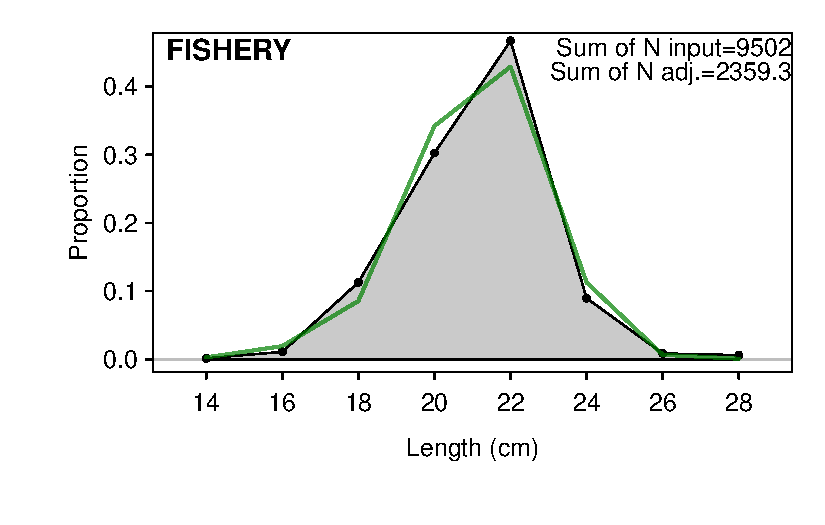
\includegraphics{LUKA_50_Base_model_diags_report_files/figure-pdf/lencompfits-1.pdf}

}

\end{figure}

\begin{figure}

{\centering 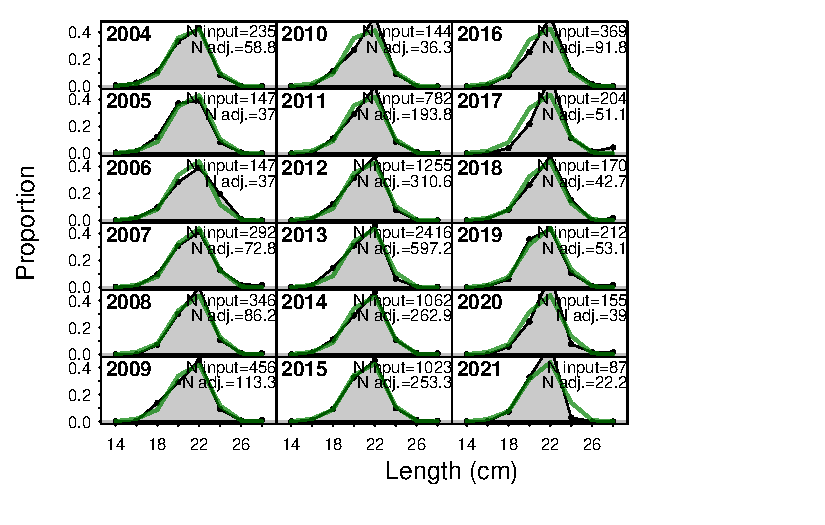
\includegraphics{LUKA_50_Base_model_diags_report_files/figure-pdf/lencompfits-2.pdf}

}

\end{figure}

\hypertarget{retrospective-and-hindcasting}{%
\paragraph{Retrospective and
Hindcasting}\label{retrospective-and-hindcasting}}

\hypertarget{retrospective}{%
\subsubsection{Retrospective}\label{retrospective}}

\begin{verbatim}
Mohn's Rho stats, including one step ahead forecasts:
\end{verbatim}

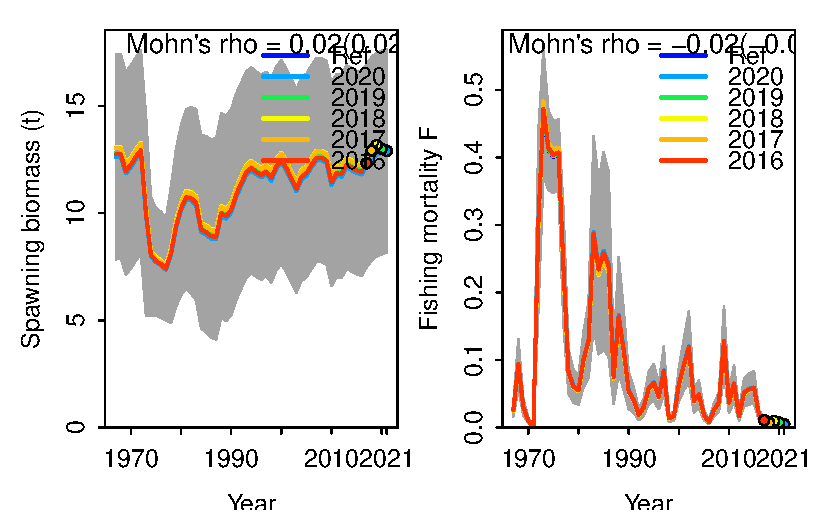
\includegraphics{LUKA_50_Base_model_diags_report_files/figure-pdf/retrospectives-1.pdf}

\begin{verbatim}
Mohn's Rho stats, including one step ahead forecasts:
\end{verbatim}

\begin{verbatim}
  type     peel          Rho  ForecastRho
1    F     2020  0.001090502  0.001085840
2    F     2019 -0.013996490 -0.013750219
3    F     2018 -0.032368650 -0.031540687
4    F     2017 -0.027841637 -0.026640244
5    F     2016 -0.007909789 -0.007532871
6    F Combined -0.016205213 -0.015675636
\end{verbatim}

\hypertarget{hindcasting}{%
\subsubsection{Hindcasting}\label{hindcasting}}

\begin{verbatim}
Plotting Hindcast Cross-Validation (one-step-ahead) 

 Computing MASE with only 4 of 5  prediction residuals for Index FISHERY 

 Warning:  Unequal spacing of naive predictions residuals may influence the interpretation of MASE 
\end{verbatim}

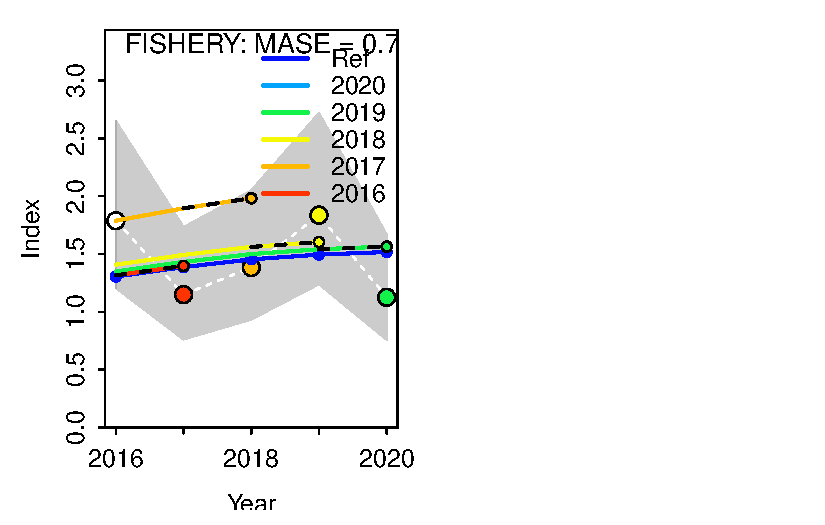
\includegraphics{LUKA_50_Base_model_diags_report_files/figure-pdf/hindcast-1.pdf}

\begin{verbatim}

MASE stats by Index:
Plotting Hindcast Cross-Validation (one-step-ahead) 

 Computing MASE with only 4 of 5  prediction residuals for Index FISHERY 

 Warning:  Unequal spacing of naive predictions residuals may influence the interpretation of MASE 
\end{verbatim}

\begin{verbatim}

MASE stats by Index:
\end{verbatim}

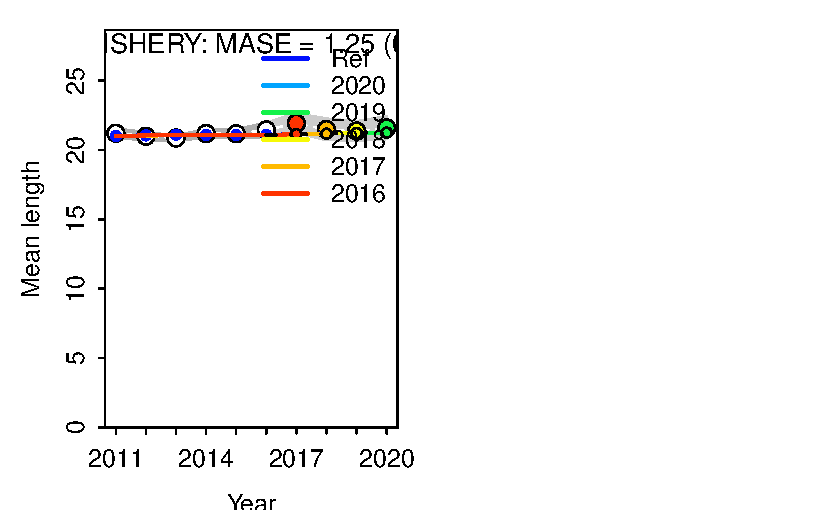
\includegraphics{LUKA_50_Base_model_diags_report_files/figure-pdf/hindcast-2.pdf}

\hypertarget{recruitment-deviations}{%
\paragraph{Recruitment Deviations}\label{recruitment-deviations}}

\hypertarget{likelihood-profile}{%
\paragraph{Likelihood Profile}\label{likelihood-profile}}

\begin{verbatim}
[1] "SR_LN"
                     frac_change include                            label
TOTAL                     1.0000    TRUE                            Total
Catch                     0.7725    TRUE                            Catch
Equil_catch               0.0034   FALSE                Equilibrium catch
Survey                    0.0557    TRUE                       Index data
Length_comp               0.2089    TRUE                      Length data
Recruitment               0.0000   FALSE                      Recruitment
InitEQ_Regime             0.0000   FALSE Initital equilibrium recruitment
Forecast_Recruitment      0.0000   FALSE             Forecast recruitment
Parm_priors               0.0006   FALSE                           Priors
Parm_softbounds           0.0000   FALSE                      Soft bounds
Parm_devs                 0.0000   FALSE             Parameter deviations
Crash_Pen                 0.0000   FALSE                    Crash penalty
\end{verbatim}

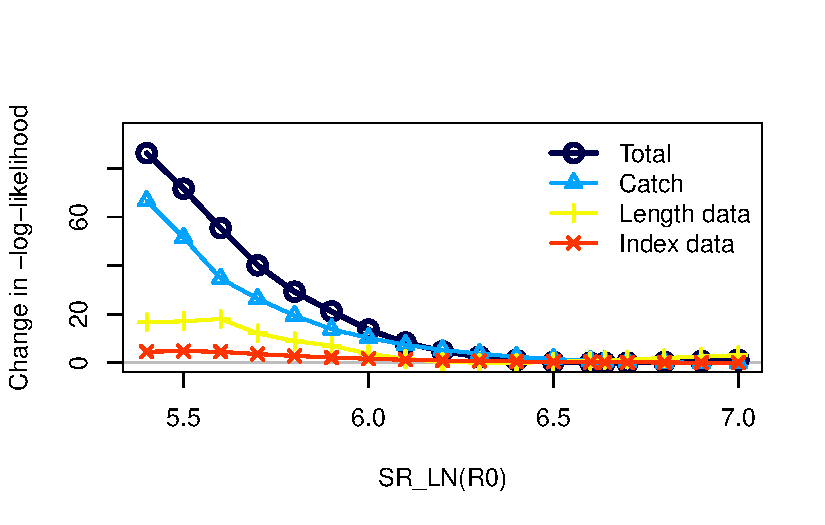
\includegraphics{LUKA_50_Base_model_diags_report_files/figure-pdf/r0prof-1.pdf}

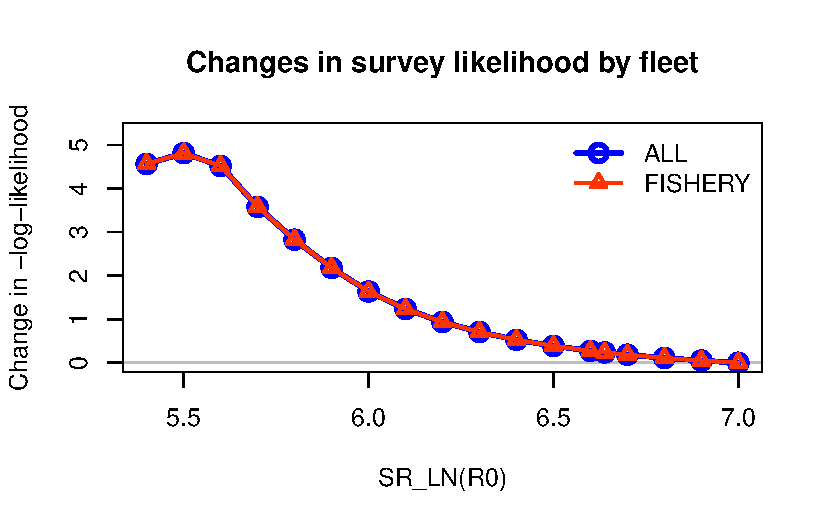
\includegraphics{LUKA_50_Base_model_diags_report_files/figure-pdf/r0prof-2.pdf}

\hypertarget{management-quantities}{%
\paragraph{Management Quantities}\label{management-quantities}}

\begin{verbatim}

 starter.sso with Bratio: SSB/SSBMSY and F: _abs_F 
 
\end{verbatim}

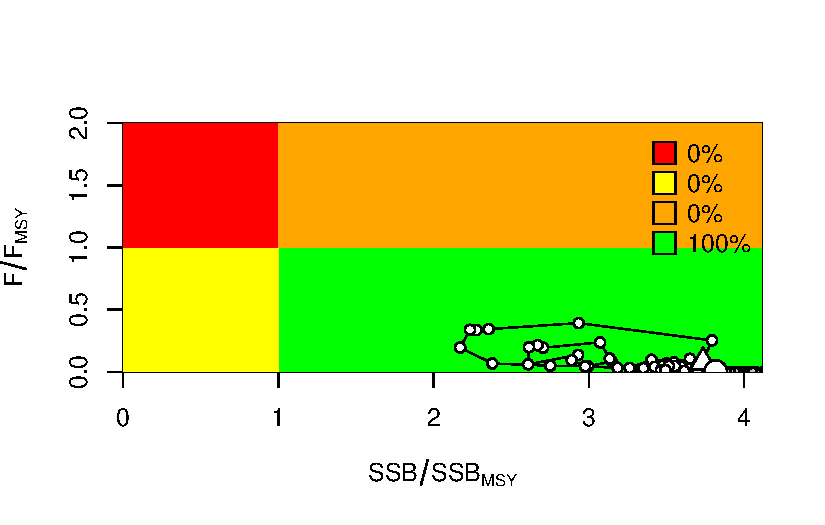
\includegraphics{LUKA_50_Base_model_diags_report_files/figure-pdf/mvlnkb-1.pdf}

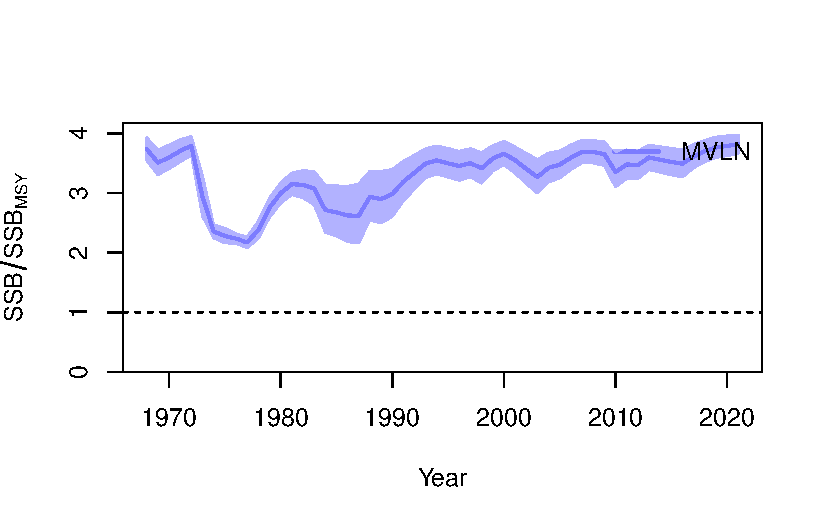
\includegraphics{LUKA_50_Base_model_diags_report_files/figure-pdf/mvlnkb-2.pdf}

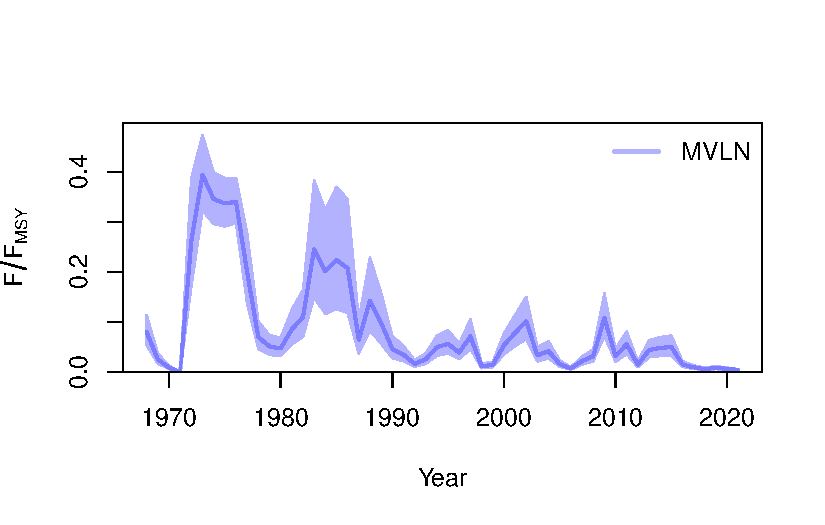
\includegraphics{LUKA_50_Base_model_diags_report_files/figure-pdf/mvlnkb-3.pdf}

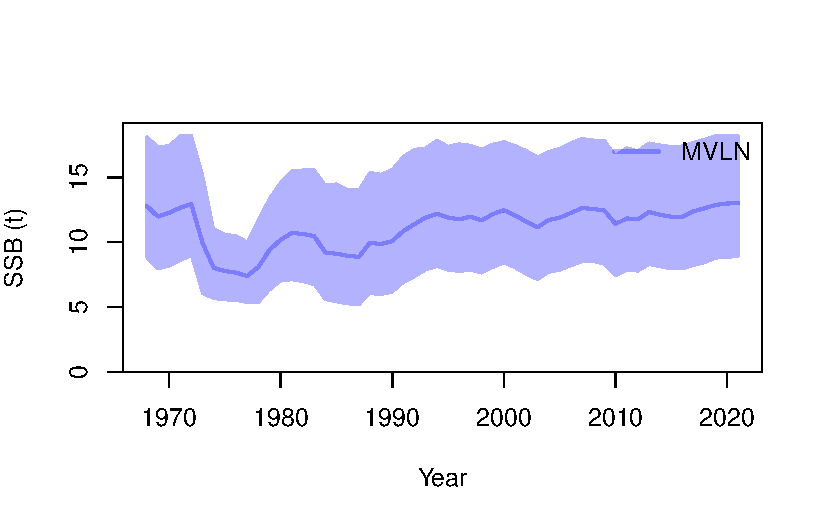
\includegraphics{LUKA_50_Base_model_diags_report_files/figure-pdf/mvlnkb-4.pdf}

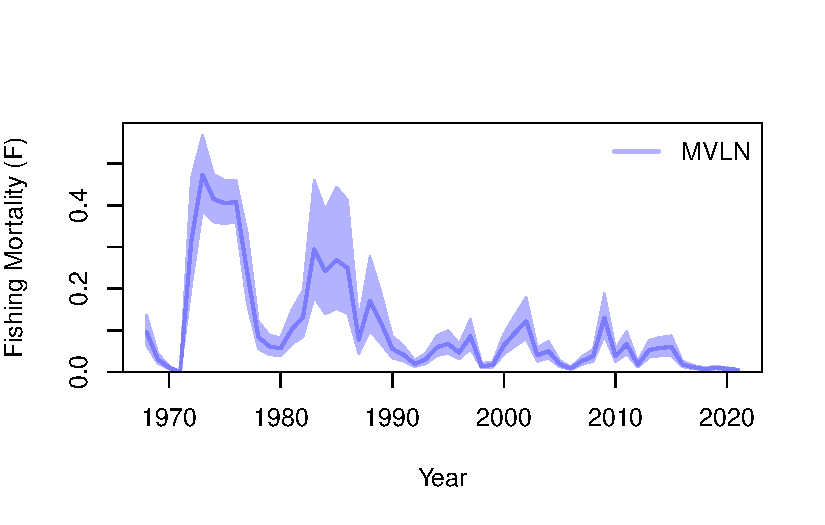
\includegraphics{LUKA_50_Base_model_diags_report_files/figure-pdf/mvlnkb-5.pdf}

\begin{verbatim}
null device 
          1 
\end{verbatim}

\hypertarget{jitter}{%
\paragraph{Jitter}\label{jitter}}

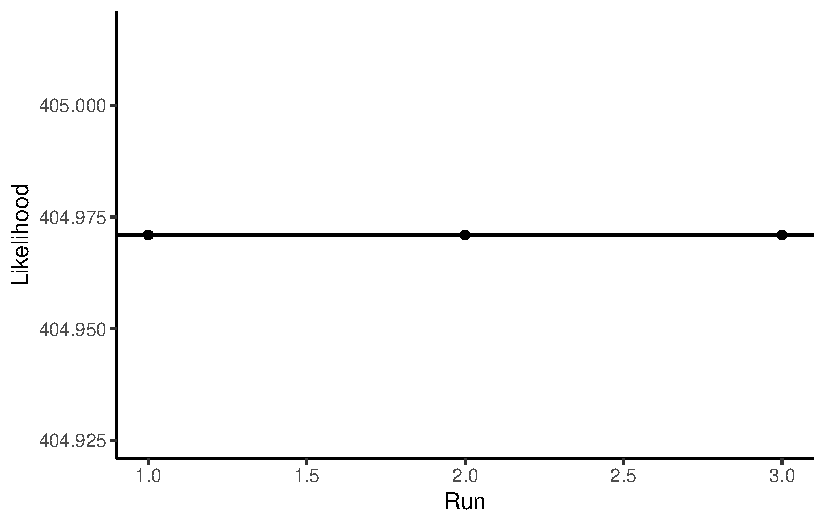
\includegraphics{LUKA_50_Base_model_diags_report_files/figure-pdf/jitter-1.pdf}

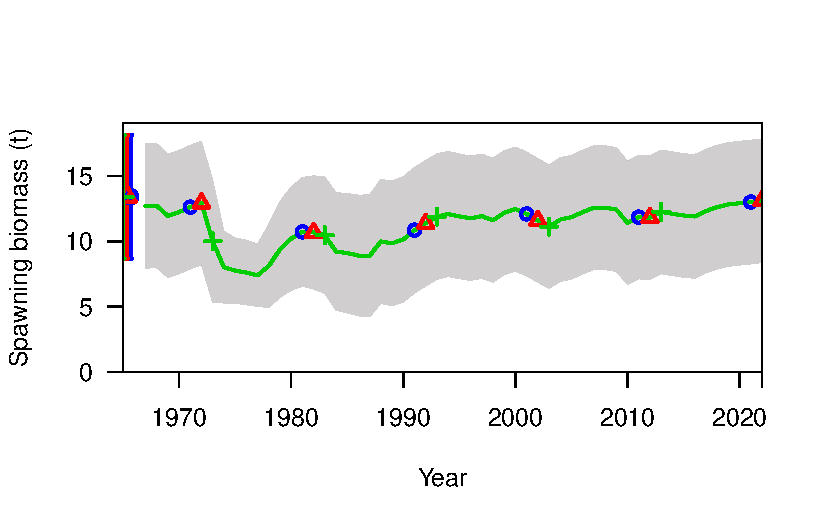
\includegraphics{LUKA_50_Base_model_diags_report_files/figure-pdf/model-comparisons-1.pdf}

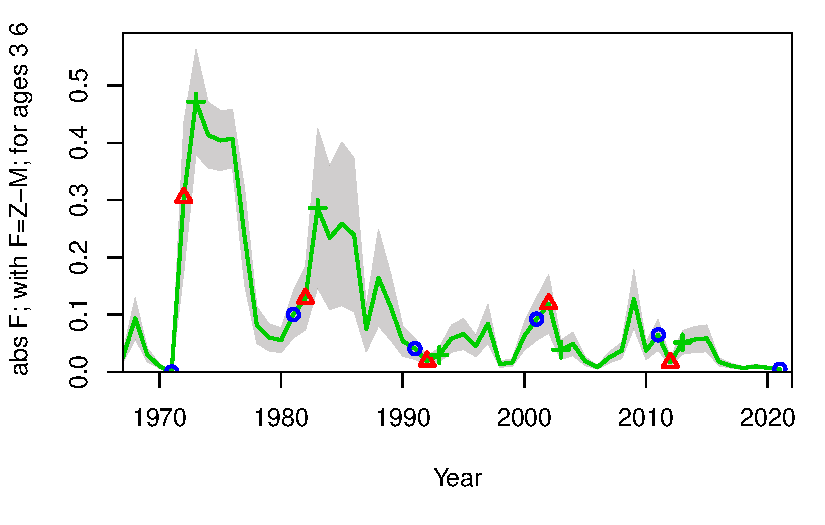
\includegraphics{LUKA_50_Base_model_diags_report_files/figure-pdf/model-comparisons-2.pdf}

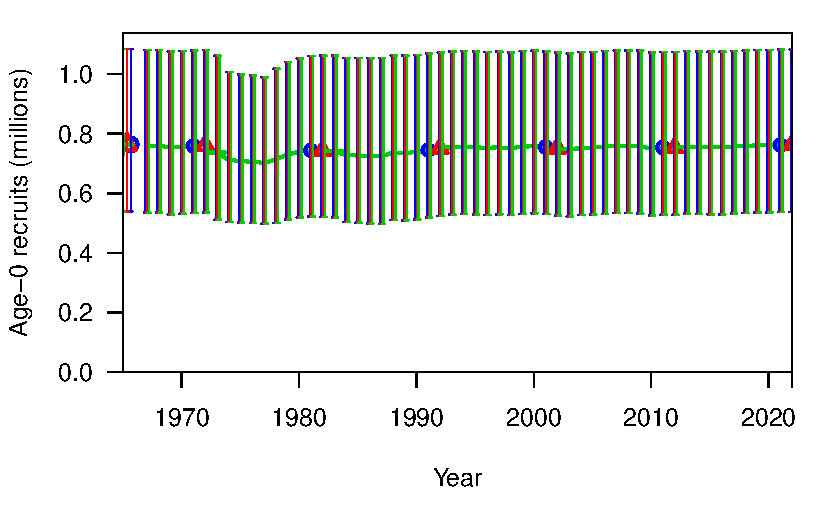
\includegraphics{LUKA_50_Base_model_diags_report_files/figure-pdf/model-comparisons-3.pdf}

\hypertarget{selectivity-and-maturity}{%
\paragraph{Selectivity and Maturity}\label{selectivity-and-maturity}}

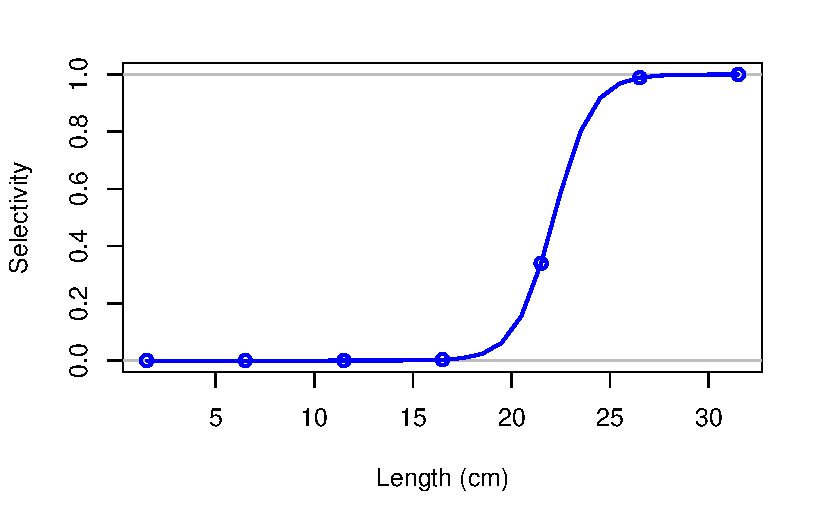
\includegraphics[width=7.4cm,height=\textheight]{LUKA_50_Base_model_diags_report_files/figure-pdf/selectivity-1.pdf}

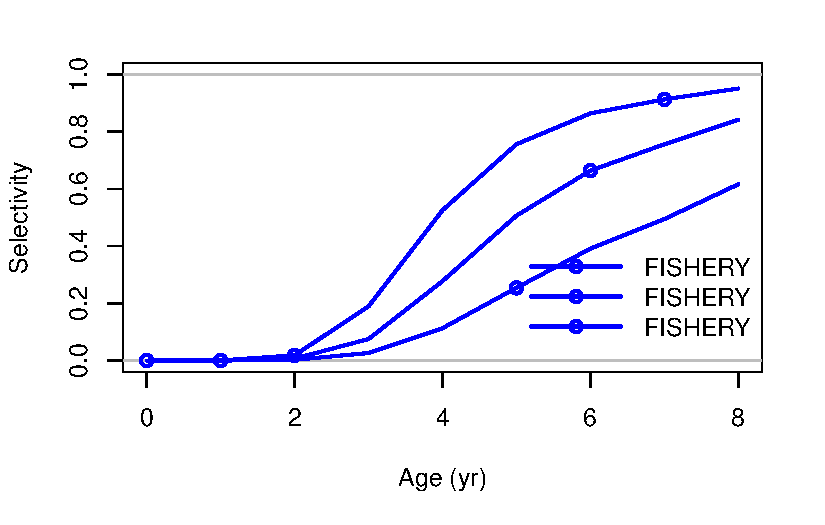
\includegraphics[width=7.4cm,height=\textheight]{LUKA_50_Base_model_diags_report_files/figure-pdf/selectivity-2.pdf}

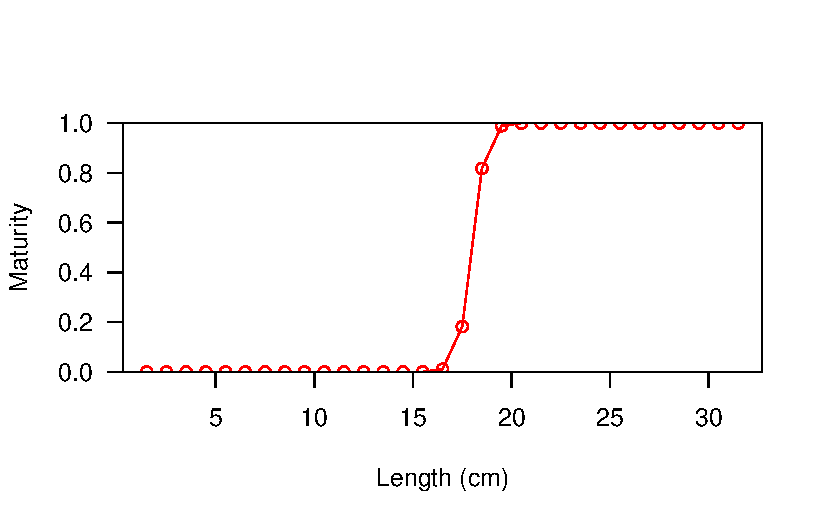
\includegraphics[width=7.2cm,height=\textheight]{LUKA_50_Base_model_diags_report_files/figure-pdf/maturity-1.pdf}

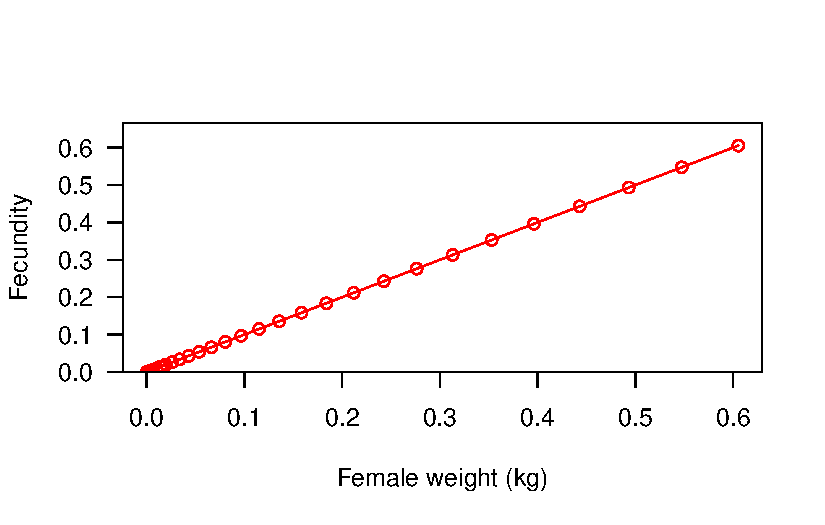
\includegraphics[width=7.2cm,height=\textheight]{LUKA_50_Base_model_diags_report_files/figure-pdf/maturity-2.pdf}



\end{document}
